\documentclass[8pt,aspectratio=169]{beamer}
\usetheme{Madrid}
\usepackage{graphicx}
\usepackage{booktabs}
\usepackage{adjustbox}
\usepackage{multicol}
\usepackage{amsmath}
\usepackage{amssymb}
\usepackage{listings}
\usepackage{xcolor}

% Color definitions
\definecolor{mlblue}{RGB}{0,102,204}
\definecolor{mlpurple}{RGB}{51,51,178}
\definecolor{mllavender}{RGB}{173,173,224}
\definecolor{mllavender2}{RGB}{193,193,232}
\definecolor{mllavender3}{RGB}{204,204,235}
\definecolor{mllavender4}{RGB}{214,214,239}
\definecolor{mlorange}{RGB}{255, 127, 14}
\definecolor{mlgreen}{RGB}{44, 160, 44}
\definecolor{mlred}{RGB}{214, 39, 40}
\definecolor{mlgray}{RGB}{127, 127, 127}

% Additional colors for template compatibility
\definecolor{lightgray}{RGB}{240, 240, 240}
\definecolor{midgray}{RGB}{180, 180, 180}

% Apply custom colors to Madrid theme
\setbeamercolor{palette primary}{bg=mllavender3,fg=mlpurple}
\setbeamercolor{palette secondary}{bg=mllavender2,fg=mlpurple}
\setbeamercolor{palette tertiary}{bg=mllavender,fg=white}
\setbeamercolor{palette quaternary}{bg=mlpurple,fg=white}

\setbeamercolor{structure}{fg=mlpurple}
\setbeamercolor{section in toc}{fg=mlpurple}
\setbeamercolor{subsection in toc}{fg=mlblue}
\setbeamercolor{title}{fg=mlpurple}
\setbeamercolor{frametitle}{fg=mlpurple,bg=mllavender3}
\setbeamercolor{block title}{bg=mllavender2,fg=mlpurple}
\setbeamercolor{block body}{bg=mllavender4,fg=black}

% Remove navigation symbols
\setbeamertemplate{navigation symbols}{}

% Clean itemize/enumerate
\setbeamertemplate{itemize items}[circle]
\setbeamertemplate{enumerate items}[default]

% Reduce margins for more content space
\setbeamersize{text margin left=5mm,text margin right=5mm}

% Command for bottom annotation (Madrid-style)
\newcommand{\bottomnote}[1]{%
\vfill
\vspace{-2mm}
\textcolor{mllavender2}{\rule{\textwidth}{0.4pt}}
\vspace{1mm}
\footnotesize
\textbf{#1}
}

% TikZ and pgfplots packages
\usepackage{tikz}
\usepackage{pgfplots}
\pgfplotsset{compat=1.18}
\usetikzlibrary{arrows.meta, positioning, shapes.geometric, shapes.symbols, calc, decorations.pathmorphing}

\title{Cryptography for Blockchain: A Visual Introduction}
\subtitle{Standalone Mini-Lecture}
\author{Prof.~Dr.~Joerg Osterrieder}
\institute{University Lecture Series}
\date{\today}

\begin{document}

% ==================== FRAME 1: TITLE ====================
\begin{frame}[plain]
\vspace{2cm}
\begin{center}
{\Huge\color{mlpurple} Cryptography for Blockchain}\\[0.4cm]
{\Large\color{mlblue} A Visual Introduction}\\[0.3cm]
{\normalsize Standalone Mini-Lecture}\\[0.3cm]
\textcolor{mlgray}{\rule{6cm}{0.4pt}}\\[0.3cm]
{\small\itshape ``Don't trust -- verify mathematically''}\\[1.5cm]
{\normalsize Prof.~Dr.~Joerg Osterrieder}\\[0.2cm]
{\small University Lecture Series}\\[0.2cm]
{\small \today}
\end{center}
\end{frame}

% ==================== FRAME 2: THE SECRET MESSAGE PROBLEM (Comic Strip 1) ====================
\begin{frame}{The Secret Message Problem}
\begin{center}
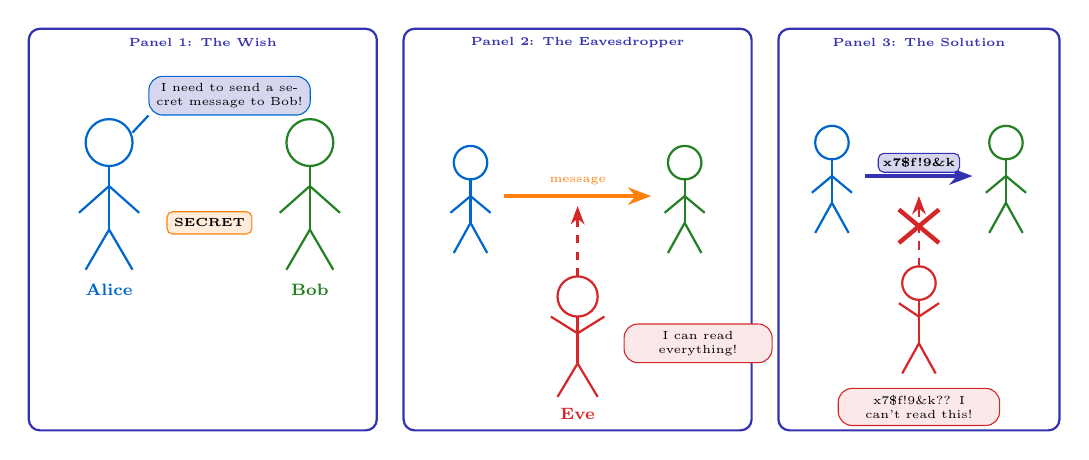
\begin{tikzpicture}[scale=0.85, every node/.style={transform shape}]

% --- Panel 1: Alice wants to send a message ---
\draw[mlpurple, thick, rounded corners=4pt] (-7.2,-2.8) rectangle (-2.0,3.2);
\node[font=\tiny\bfseries, mlpurple] at (-4.6,3.0) {Panel 1: The Wish};

% Alice stick figure
\draw[mlblue, thick] (-6.0,1.5) circle (0.35);
\draw[mlblue, thick] (-6.0,1.15) -- (-6.0,0.2);
\draw[mlblue, thick] (-6.0,0.85) -- (-6.45,0.45);
\draw[mlblue, thick] (-6.0,0.85) -- (-5.55,0.45);
\draw[mlblue, thick] (-6.0,0.2) -- (-6.35,-0.4);
\draw[mlblue, thick] (-6.0,0.2) -- (-5.65,-0.4);
\node[font=\scriptsize\bfseries, mlblue] at (-6.0,-0.7) {Alice};

% Alice speech bubble
\node[draw=mlblue, fill=mllavender4, rounded corners=5pt, font=\tiny,
      text width=2.2cm, align=center, inner sep=3pt]
      (alice-bubble1) at (-4.2,2.2) {I need to send a secret message to Bob!};
\draw[mlblue, thick] (-5.65,1.65) -- (alice-bubble1.south west);

% Letter icon between them
\node[draw=mlorange, fill=mlorange!15, rounded corners=2pt, font=\tiny\bfseries,
      inner sep=3pt] at (-4.5,0.3) {SECRET};

% Bob stick figure
\draw[mlgreen!80!black, thick] (-3.0,1.5) circle (0.35);
\draw[mlgreen!80!black, thick] (-3.0,1.15) -- (-3.0,0.2);
\draw[mlgreen!80!black, thick] (-3.0,0.85) -- (-3.45,0.45);
\draw[mlgreen!80!black, thick] (-3.0,0.85) -- (-2.55,0.45);
\draw[mlgreen!80!black, thick] (-3.0,0.2) -- (-3.35,-0.4);
\draw[mlgreen!80!black, thick] (-3.0,0.2) -- (-2.65,-0.4);
\node[font=\scriptsize\bfseries, mlgreen!80!black] at (-3.0,-0.7) {Bob};

% --- Panel 2: Eve is eavesdropping ---
\draw[mlpurple, thick, rounded corners=4pt] (-1.6,-2.8) rectangle (3.6,3.2);
\node[font=\tiny\bfseries, mlpurple] at (1.0,3.0) {Panel 2: The Eavesdropper};

% Alice (small) sending message
\draw[mlblue, thick] (-0.6,1.2) circle (0.25);
\draw[mlblue, thick] (-0.6,0.95) -- (-0.6,0.3);
\draw[mlblue, thick] (-0.6,0.7) -- (-0.9,0.45);
\draw[mlblue, thick] (-0.6,0.7) -- (-0.3,0.45);
\draw[mlblue, thick] (-0.6,0.3) -- (-0.85,-0.15);
\draw[mlblue, thick] (-0.6,0.3) -- (-0.35,-0.15);

% Bob (small)
\draw[mlgreen!80!black, thick] (2.6,1.2) circle (0.25);
\draw[mlgreen!80!black, thick] (2.6,0.95) -- (2.6,0.3);
\draw[mlgreen!80!black, thick] (2.6,0.7) -- (2.3,0.45);
\draw[mlgreen!80!black, thick] (2.6,0.7) -- (2.9,0.45);
\draw[mlgreen!80!black, thick] (2.6,0.3) -- (2.35,-0.15);
\draw[mlgreen!80!black, thick] (2.6,0.3) -- (2.85,-0.15);

% Message arrow
\draw[-{Stealth}, mlorange, very thick] (-0.1,0.7) -- (2.1,0.7);
\node[font=\tiny, mlorange, above] at (1.0,0.75) {message};

% Eve stick figure (lurking below)
\draw[mlred, thick] (1.0,-0.8) circle (0.3);
\draw[mlred, thick] (1.0,-1.1) -- (1.0,-1.8);
\draw[mlred, thick] (1.0,-1.35) -- (0.6,-1.1);
\draw[mlred, thick] (1.0,-1.35) -- (1.4,-1.1);
\draw[mlred, thick] (1.0,-1.8) -- (0.7,-2.3);
\draw[mlred, thick] (1.0,-1.8) -- (1.3,-2.3);
\node[font=\scriptsize\bfseries, mlred] at (1.0,-2.55) {Eve};

% Eve's interception arrow
\draw[-{Stealth}, mlred, thick, dashed] (1.0,-0.5) -- (1.0,0.55);

% Eve speech bubble
\node[draw=mlred, fill=mlred!10, rounded corners=5pt, font=\tiny,
      text width=2.0cm, align=center, inner sep=3pt]
      at (2.8,-1.5) {I can read everything!};

% --- Panel 3: The cryptographic solution ---
\draw[mlpurple, thick, rounded corners=4pt] (4.0,-2.8) rectangle (8.2,3.2);
\node[font=\tiny\bfseries, mlpurple] at (6.1,3.0) {Panel 3: The Solution};

% Alice sending encrypted message
\draw[mlblue, thick] (4.8,1.5) circle (0.25);
\draw[mlblue, thick] (4.8,1.25) -- (4.8,0.6);
\draw[mlblue, thick] (4.8,1.0) -- (4.5,0.75);
\draw[mlblue, thick] (4.8,1.0) -- (5.1,0.75);
\draw[mlblue, thick] (4.8,0.6) -- (4.55,0.15);
\draw[mlblue, thick] (4.8,0.6) -- (5.05,0.15);

% Bob receiving
\draw[mlgreen!80!black, thick] (7.4,1.5) circle (0.25);
\draw[mlgreen!80!black, thick] (7.4,1.25) -- (7.4,0.6);
\draw[mlgreen!80!black, thick] (7.4,1.0) -- (7.1,0.75);
\draw[mlgreen!80!black, thick] (7.4,1.0) -- (7.7,0.75);
\draw[mlgreen!80!black, thick] (7.4,0.6) -- (7.15,0.15);
\draw[mlgreen!80!black, thick] (7.4,0.6) -- (7.65,0.15);

% Encrypted message arrow
\draw[-{Stealth}, mlpurple, very thick] (5.3,1.0) -- (6.9,1.0);
\node[draw=mlpurple, fill=mllavender4, font=\tiny\bfseries, inner sep=2pt,
      rounded corners=2pt, above] at (6.1,1.05) {x7\$f!9\&k};

% Eve below, confused
\draw[mlred, thick] (6.1,-0.6) circle (0.25);
\draw[mlred, thick] (6.1,-0.85) -- (6.1,-1.5);
\draw[mlred, thick] (6.1,-1.1) -- (5.8,-0.9);
\draw[mlred, thick] (6.1,-1.1) -- (6.4,-0.9);
\draw[mlred, thick] (6.1,-1.5) -- (5.85,-1.95);
\draw[mlred, thick] (6.1,-1.5) -- (6.35,-1.95);

% Eve confused bubble
\node[draw=mlred, fill=mlred!10, rounded corners=5pt, font=\tiny,
      text width=2.2cm, align=center, inner sep=3pt]
      at (6.1,-2.45) {x7\$f!9\&k?? I can't read this!};

% Crossed-out interception arrow
\draw[-{Stealth}, mlred, thick, dashed] (6.1,-0.35) -- (6.1,0.7);
\draw[mlred, ultra thick] (5.8,0.0) -- (6.4,0.5);
\draw[mlred, ultra thick] (5.8,0.5) -- (6.4,0.0);

\end{tikzpicture}
\end{center}
\bottomnote{Cryptography lets Alice and Bob communicate securely even when Eve controls the channel.}
\end{frame}

% ==================== FRAME 3: ONE-WAY FUNCTIONS -- THE MEAT GRINDER (Comic Strip 2) ====================
\begin{frame}{One-Way Functions: The Meat Grinder}
\begin{center}
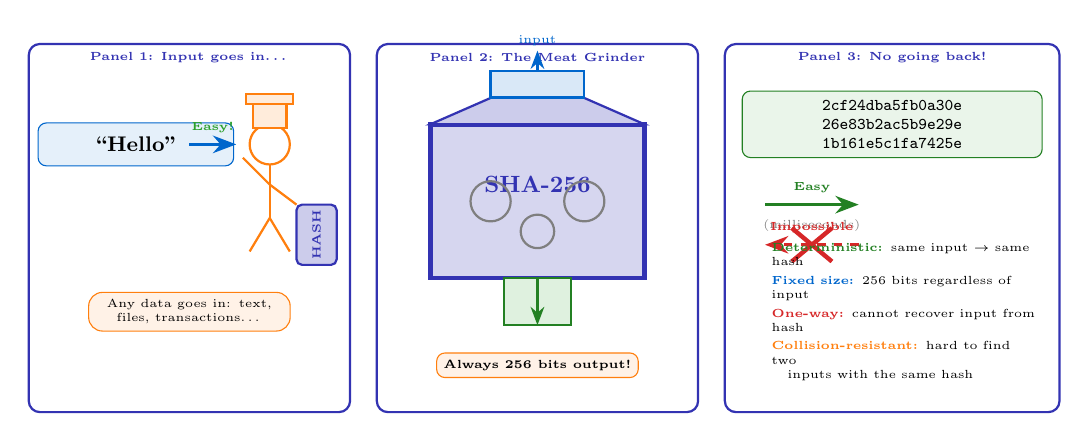
\begin{tikzpicture}[scale=0.85, every node/.style={transform shape}]

% --- Panel 1: The input ---
\draw[mlpurple, thick, rounded corners=4pt] (-7.2,-2.5) rectangle (-2.4,3.0);
\node[font=\tiny\bfseries, mlpurple] at (-4.8,2.8) {Panel 1: Input goes in\ldots};

% Input document
\node[draw=mlblue, fill=mlblue!10, rounded corners=3pt, font=\small\bfseries,
      inner sep=6pt, text width=2.5cm, align=center] (input) at (-5.6,1.5) {``Hello''};

% Chef stick figure feeding the grinder
\draw[mlorange, thick] (-3.6,1.5) circle (0.3);
\draw[mlorange, thick] (-3.6,1.2) -- (-3.6,0.4);
\draw[mlorange, thick] (-3.6,0.9) -- (-4.0,1.3);
\draw[mlorange, thick] (-3.6,0.9) -- (-3.2,0.6);
\draw[mlorange, thick] (-3.6,0.4) -- (-3.9,-0.1);
\draw[mlorange, thick] (-3.6,0.4) -- (-3.3,-0.1);
% Chef hat
\draw[mlorange, thick, fill=mlorange!15] (-3.85,1.75) rectangle (-3.35,2.1);
\draw[mlorange, thick, fill=mlorange!15] (-3.95,2.1) rectangle (-3.25,2.25);

% Arrow: input to grinder
\draw[-{Stealth}, mlblue, very thick] (-4.8,1.5) -- (-4.1,1.5);
\node[font=\tiny\bfseries, mlgreen, above] at (-4.45,1.55) {Easy!};

% Speech bubble
\node[draw=mlorange, fill=mlorange!10, rounded corners=5pt, font=\tiny,
      text width=2.8cm, align=center, inner sep=3pt]
      at (-4.8,-1.0) {Any data goes in: text, files, transactions\ldots};

% Grinder machine
\draw[mlpurple, thick, fill=mllavender3, rounded corners=2pt]
     (-3.2,-0.3) rectangle (-2.6,0.6);
\node[font=\tiny\bfseries, mlpurple, rotate=90] at (-2.9,0.15) {HASH};

% --- Panel 2: The grinder (SHA-256) ---
\draw[mlpurple, thick, rounded corners=4pt] (-2.0,-2.5) rectangle (2.8,3.0);
\node[font=\tiny\bfseries, mlpurple] at (0.4,2.8) {Panel 2: The Meat Grinder};

% Large grinder illustration
\draw[mlpurple, ultra thick, fill=mllavender4] (-1.2,-0.5) rectangle (2.0,1.8);
\draw[mlpurple, thick, fill=mllavender3] (-1.2,1.8) -- (0.4,2.5) -- (2.0,1.8) -- cycle;
\node[font=\normalsize\bfseries, mlpurple] at (0.4,0.9) {SHA-256};

% Input hopper (top)
\draw[mlblue, thick, fill=mlblue!15] (-0.3,2.2) rectangle (1.1,2.6);
\draw[-{Stealth}, mlblue, thick] (0.4,2.6) -- (0.4,2.9);
\node[font=\tiny, mlblue] at (0.4,3.05) {input};

% Output chute (bottom)
\draw[mlgreen!80!black, thick, fill=mlgreen!15] (-0.1,-1.2) rectangle (0.9,-0.5);
\draw[-{Stealth}, mlgreen!80!black, thick] (0.4,-0.5) -- (0.4,-1.2);

% Gears inside
\draw[mlgray, thick] (-0.3,0.65) circle (0.3);
\draw[mlgray, thick] (1.1,0.65) circle (0.3);
\draw[mlgray, thick] (0.4,0.2) circle (0.25);

% Always 256 bits label
\node[draw=mlorange, fill=mlorange!10, rounded corners=3pt,
      font=\tiny\bfseries, inner sep=3pt] at (0.4,-1.8) {Always 256 bits output!};

% --- Panel 3: Output and irreversibility ---
\draw[mlpurple, thick, rounded corners=4pt] (3.2,-2.5) rectangle (8.2,3.0);
\node[font=\tiny\bfseries, mlpurple] at (5.7,2.8) {Panel 3: No going back!};

% Output hash
\node[draw=mlgreen!80!black, fill=mlgreen!10, rounded corners=3pt,
      font=\scriptsize\ttfamily, inner sep=4pt, text width=4.2cm, align=center]
      (output) at (5.7,1.8) {2cf24dba5fb0a30e\\26e83b2ac5b9e29e\\1b161e5c1fa7425e};

% Forward arrow: easy
\draw[-{Stealth}, mlgreen!80!black, very thick] (3.8,0.6) -- (5.2,0.6);
\node[font=\tiny\bfseries, mlgreen!80!black, above] at (4.5,0.65) {Easy};
\node[font=\tiny, mlgray, below] at (4.5,0.5) {(milliseconds)};

% Reverse arrow: impossible
\draw[-{Stealth}, mlred, very thick, dashed] (5.2,0.0) -- (3.8,0.0);
\node[font=\tiny\bfseries, mlred, above] at (4.5,0.05) {Impossible};
\draw[mlred, ultra thick] (4.2,-0.25) -- (4.8,0.25);
\draw[mlred, ultra thick] (4.2,0.25) -- (4.8,-0.25);

% Properties list
\node[font=\tiny, align=left, text width=4cm] at (5.9,-1.0) {%
\textcolor{mlgreen!80!black}{\bfseries Deterministic:} same input $\to$ same hash\\[2pt]
\textcolor{mlblue}{\bfseries Fixed size:} 256 bits regardless of input\\[2pt]
\textcolor{mlred}{\bfseries One-way:} cannot recover input from hash\\[2pt]
\textcolor{mlorange}{\bfseries Collision-resistant:} hard to find two\\
\hspace{1em}inputs with the same hash};

\end{tikzpicture}
\end{center}
\bottomnote{SHA-256 is Bitcoin's hash function. It produces a unique 256-bit ``fingerprint'' for any input.}
\end{frame}

% ==================== FRAME 4: THE AVALANCHE EFFECT ====================
\begin{frame}{The Avalanche Effect}
\begin{columns}[T]
\begin{column}{0.55\textwidth}
\begin{center}
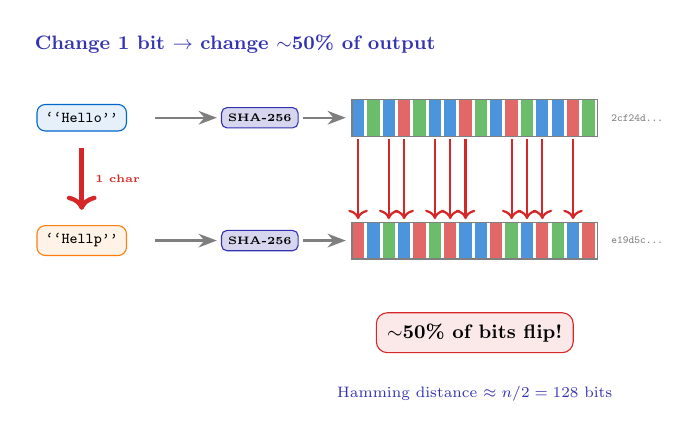
\begin{tikzpicture}[scale=0.78, every node/.style={transform shape}]

% Title
\node[font=\small\bfseries, mlpurple] at (0,4.2) {Change 1 bit $\to$ change $\sim$50\% of output};

% --- Path 1: original input ---
\node[draw=mlblue, fill=mlblue!10, rounded corners=3pt, font=\scriptsize\ttfamily,
      inner sep=4pt] (in1) at (-2.5,3.0) {``Hello''};

\draw[-{Stealth}, mlgray, thick] (-1.3,3.0) -- (-0.3,3.0);

\node[draw=mlpurple, fill=mllavender4, rounded corners=2pt,
      font=\tiny\bfseries, inner sep=3pt] (sha1) at (0.4,3.0) {SHA-256};

\draw[-{Stealth}, mlgray, thick] (1.1,3.0) -- (1.8,3.0);

% Hash output as colored bit strip
\foreach \i/\c in {0/mlblue,1/mlgreen,2/mlblue,3/mlred,4/mlgreen,
                    5/mlblue,6/mlblue,7/mlred,8/mlgreen,9/mlblue,
                    10/mlred,11/mlgreen,12/mlblue,13/mlblue,14/mlred,15/mlgreen} {
  \fill[\c!70] (1.9+\i*0.25,2.7) rectangle (2.1+\i*0.25,3.3);
}
\draw[mlgray, thin] (1.9,2.7) rectangle (5.9,3.3);
\node[font=\tiny\ttfamily, mlgray, right] at (6.0,3.0) {2cf24d\ldots};

% --- Path 2: modified input (1 char different) ---
\node[draw=mlorange, fill=mlorange!10, rounded corners=3pt, font=\scriptsize\ttfamily,
      inner sep=4pt] (in2) at (-2.5,1.0) {``Hellp''};

\draw[-{Stealth}, mlgray, thick] (-1.3,1.0) -- (-0.3,1.0);

\node[draw=mlpurple, fill=mllavender4, rounded corners=2pt,
      font=\tiny\bfseries, inner sep=3pt] (sha2) at (0.4,1.0) {SHA-256};

\draw[-{Stealth}, mlgray, thick] (1.1,1.0) -- (1.8,1.0);

% Hash output as colored bit strip (very different)
\foreach \i/\c in {0/mlred,1/mlblue,2/mlgreen,3/mlblue,4/mlred,
                    5/mlgreen,6/mlred,7/mlblue,8/mlblue,9/mlred,
                    10/mlgreen,11/mlblue,12/mlred,13/mlgreen,14/mlblue,15/mlred} {
  \fill[\c!70] (1.9+\i*0.25,0.7) rectangle (2.1+\i*0.25,1.3);
}
\draw[mlgray, thin] (1.9,0.7) rectangle (5.9,1.3);
\node[font=\tiny\ttfamily, mlgray, right] at (6.0,1.0) {e19d5c\ldots};

% Highlight the 1-char difference
\draw[mlred, ultra thick, ->] (-2.5,2.5) -- (-2.5,1.5);
\node[font=\tiny\bfseries, mlred, right] at (-2.4,2.0) {1 char};

% Show bits that flipped (arrows between strips)
\foreach \i in {0,2,3,5,6,7,10,11,12,14} {
  \draw[mlred, thick, ->] (2.0+\i*0.25,2.65) -- (2.0+\i*0.25,1.35);
}

% Percentage annotation
\node[draw=mlred, fill=mlred!10, rounded corners=4pt, font=\small\bfseries,
      inner sep=5pt] at (3.9,-0.5) {$\sim$50\% of bits flip!};

% Formula
\node[font=\scriptsize, mlpurple] at (3.9,-1.5) {Hamming distance $\approx n/2 = 128$ bits};

\end{tikzpicture}
\end{center}
\end{column}
\begin{column}{0.43\textwidth}
\begin{block}{\small Why It Matters for Blockchain}
\begin{itemize}\setlength\itemsep{3pt}
\item[\textcolor{mlgreen!80!black}{\textbullet}] \textbf{Tamper detection:} Changing even one byte in a block invalidates its hash
\item[\textcolor{mlblue}{\textbullet}] \textbf{Mining puzzle:} No shortcut to find a hash starting with $k$ zeros
\item[\textcolor{mlorange}{\textbullet}] \textbf{Unpredictable:} Cannot predict output from partial input knowledge
\end{itemize}
\end{block}

\vspace{2mm}
\begin{block}{\small Formal Definition}
A hash function $H$ satisfies the \textbf{avalanche criterion} if: when a single input bit flips, each output bit flips with probability $\approx 0.5$:
\[
\Pr\bigl[\,H(x)_i \neq H(x')_i\,\bigr] \approx \tfrac{1}{2}
\]
\end{block}
\end{column}
\end{columns}
\bottomnote{The avalanche effect ensures that hash functions behave like random oracles -- no pattern leaks through.}
\end{frame}

% ==================== FRAME 5: PUBLIC & PRIVATE KEYS ====================
\begin{frame}{Public \& Private Keys}
\begin{center}
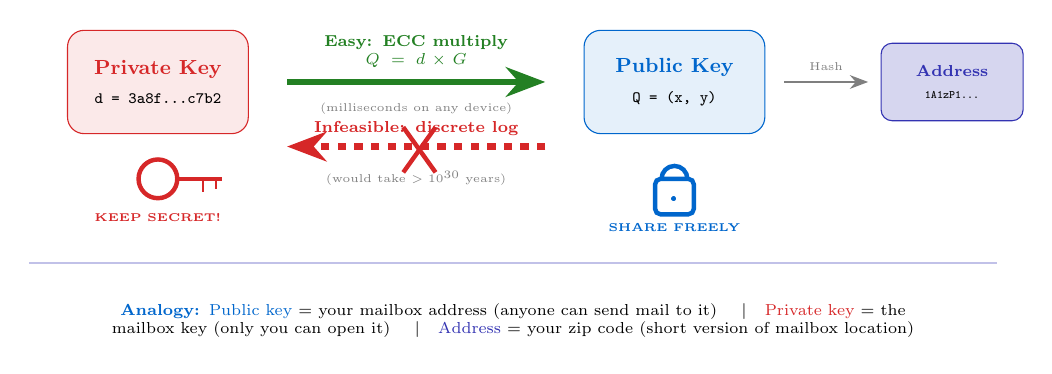
\begin{tikzpicture}[scale=0.82, every node/.style={transform shape}]

% --- Private Key (left) ---
\node[draw=mlred, fill=mlred!10, rounded corners=6pt, minimum width=2.8cm,
      minimum height=1.6cm, font=\small\bfseries, align=center] (privkey) at (-4.5,1.5)
      {\textcolor{mlred}{Private Key}\\[2pt]\scriptsize\ttfamily d = 3a8f...c7b2};

% Key icon below private key
\begin{scope}[shift={(-4.5,0.0)}]
  \draw[mlred, ultra thick] (0,0) circle (0.3);
  \draw[mlred, ultra thick] (0.3,0) -- (1.0,0);
  \draw[mlred, thick] (0.7,0) -- (0.7,-0.2);
  \draw[mlred, thick] (0.9,0) -- (0.9,-0.15);
\end{scope}
\node[font=\tiny\bfseries, mlred] at (-4.5,-0.6) {KEEP SECRET!};

% --- Arrow: easy direction (private -> public) ---
\draw[-{Stealth}, mlgreen!80!black, line width=2.5pt] (-2.5,1.5) -- (1.5,1.5);
\node[font=\scriptsize\bfseries, mlgreen!80!black, above, text width=3cm, align=center]
     at (-0.5,1.6) {Easy: ECC multiply\\$Q = d \times G$};
\node[font=\tiny, mlgray, below] at (-0.5,1.3) {(milliseconds on any device)};

% --- Arrow: infeasible direction (public -> private) ---
\draw[-{Stealth}, mlred, line width=2.5pt, dashed] (1.5,0.5) -- (-2.5,0.5);
\node[font=\scriptsize\bfseries, mlred, above, text width=3.5cm, align=center]
     at (-0.5,0.55) {Infeasible: discrete log};
\node[font=\tiny, mlgray, below] at (-0.5,0.25) {(would take $> 10^{30}$ years)};

% Big X on reverse arrow
\draw[mlred, ultra thick] (-0.7,0.1) -- (-0.2,0.8);
\draw[mlred, ultra thick] (-0.7,0.8) -- (-0.2,0.1);

% --- Public Key (right) ---
\node[draw=mlblue, fill=mlblue!10, rounded corners=6pt, minimum width=2.8cm,
      minimum height=1.6cm, font=\small\bfseries, align=center] (pubkey) at (3.5,1.5)
      {\textcolor{mlblue}{Public Key}\\[2pt]\scriptsize\ttfamily Q = (x, y)};

% Lock icon below public key
\begin{scope}[shift={(3.5,-0.15)}]
  \draw[mlblue, ultra thick, rounded corners=2pt] (-0.3,-0.4) rectangle (0.3,0.15);
  \draw[mlblue, ultra thick] (-0.2,0.15) arc (180:0:0.2) ;
  \node[font=\tiny, mlblue] at (0,-0.15) {\textbullet};
\end{scope}
\node[font=\tiny\bfseries, mlblue] at (3.5,-0.75) {SHARE FREELY};

% --- Address derivation (far right) ---
\draw[-{Stealth}, mlgray, thick] (5.2,1.5) -- (6.5,1.5);
\node[font=\tiny, mlgray, above] at (5.85,1.55) {Hash};

\node[draw=mlpurple, fill=mllavender4, rounded corners=4pt, minimum width=2.2cm,
      minimum height=1.2cm, font=\scriptsize\bfseries, align=center] at (7.8,1.5)
      {\textcolor{mlpurple}{Address}\\[2pt]\tiny\ttfamily 1A1zP1...};

% --- Bottom: analogy ---
\draw[mllavender2, thick] (-6.5,-1.3) -- (8.5,-1.3);
\node[font=\scriptsize, align=center, text width=14cm] at (1.0,-2.2) {%
\textcolor{mlblue}{\bfseries Analogy:}
\textcolor{mlblue}{Public key} = your mailbox address (anyone can send mail to it)
\quad\textbar\quad
\textcolor{mlred}{Private key} = the mailbox key (only you can open it)
\quad\textbar\quad
\textcolor{mlpurple}{Address} = your zip code (short version of mailbox location)};

\end{tikzpicture}
\end{center}
\bottomnote{Elliptic Curve Cryptography (secp256k1 in Bitcoin): $Q = d \times G$ where $G$ is a generator point on the curve.}
\end{frame}

% ==================== FRAME 6: DIGITAL SIGNATURES ====================
\begin{frame}{Digital Signatures: Proving Ownership}
\begin{center}
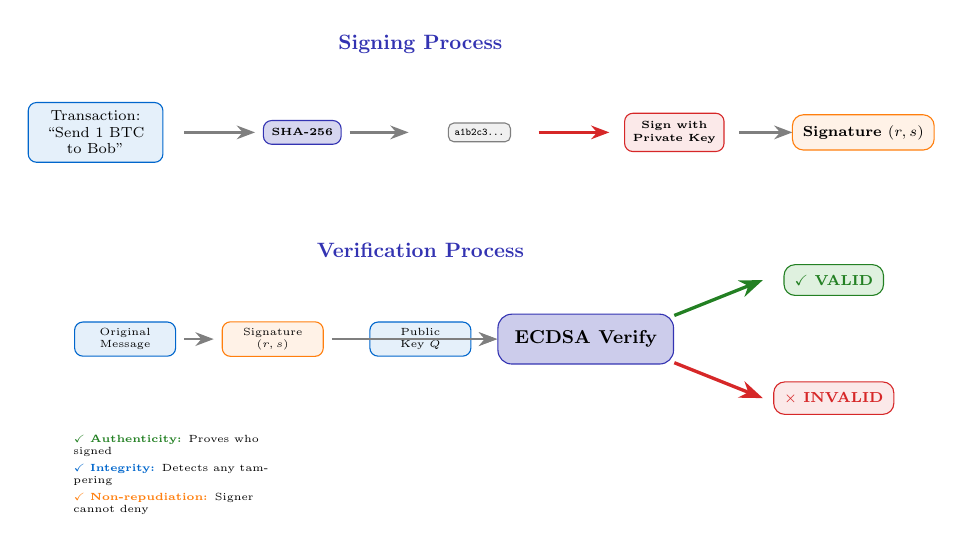
\begin{tikzpicture}[scale=0.75, every node/.style={transform shape}]

% ===== SIGNING PROCESS (Top) =====
\node[font=\normalsize\bfseries, mlpurple] at (0,4.5) {Signing Process};

% Message
\node[draw=mlblue, fill=mlblue!10, rounded corners=3pt,
      font=\scriptsize, inner sep=4pt, text width=2cm, align=center]
      (msg) at (-5.5,3.0) {Transaction:\\``Send 1 BTC\\to Bob''};

% Hash step
\draw[-{Stealth}, mlgray, thick] (-4.0,3.0) -- (-2.8,3.0);
\node[draw=mlpurple, fill=mllavender4, rounded corners=3pt,
      font=\tiny\bfseries, inner sep=4pt] (hash) at (-2.0,3.0) {SHA-256};

% Hash output
\draw[-{Stealth}, mlgray, thick] (-1.2,3.0) -- (-0.2,3.0);
\node[draw=mlgray, fill=lightgray, rounded corners=2pt,
      font=\tiny\ttfamily, inner sep=3pt] (digest) at (1.0,3.0) {a1b2c3...};

% Sign with private key
\draw[-{Stealth}, mlred, thick] (2.0,3.0) -- (3.2,3.0);
\node[draw=mlred, fill=mlred!10, rounded corners=3pt,
      font=\tiny\bfseries, inner sep=4pt, align=center] (sign) at (4.3,3.0) {Sign with\\Private Key};

% Signature output
\draw[-{Stealth}, mlgray, thick] (5.4,3.0) -- (6.3,3.0);
\node[draw=mlorange, fill=mlorange!10, rounded corners=4pt,
      font=\scriptsize\bfseries, inner sep=5pt] (sig) at (7.5,3.0) {Signature $(r, s)$};

% ===== VERIFICATION PROCESS (Bottom) =====
\node[font=\normalsize\bfseries, mlpurple] at (0,1.0) {Verification Process};

% Three inputs
\node[draw=mlblue, fill=mlblue!10, rounded corners=3pt,
      font=\tiny, inner sep=3pt, text width=1.5cm, align=center]
      (vmsg) at (-5.0,-0.5) {Original\\Message};

\node[draw=mlorange, fill=mlorange!10, rounded corners=3pt,
      font=\tiny, inner sep=3pt, text width=1.5cm, align=center]
      (vsig) at (-2.5,-0.5) {Signature\\$(r, s)$};

\node[draw=mlblue, fill=mlblue!10, rounded corners=3pt,
      font=\tiny, inner sep=3pt, text width=1.5cm, align=center]
      (vpub) at (0.0,-0.5) {Public\\Key $Q$};

% Verify box
\draw[-{Stealth}, mlgray, thick] (-4.0,-0.5) -- (-3.5,-0.5);
\draw[-{Stealth}, mlgray, thick] (-1.5,-0.5) -- (1.3,-0.5);
\draw[-{Stealth}, mlgray, thick] (0.8,-0.5) -- (1.3,-0.5);
\node[draw=mlpurple, fill=mllavender3, rounded corners=5pt,
      font=\small\bfseries, inner sep=8pt, minimum width=2.5cm]
      (verify) at (2.8,-0.5) {ECDSA Verify};

% Valid result
\draw[-{Stealth}, mlgreen!80!black, very thick] (4.3,-0.1) -- (5.8,0.5);
\node[draw=mlgreen!80!black, fill=mlgreen!15, rounded corners=4pt,
      font=\scriptsize\bfseries, inner sep=5pt] at (7.0,0.5)
      {\textcolor{mlgreen!80!black}{$\checkmark${} VALID}};

% Invalid result
\draw[-{Stealth}, mlred, very thick] (4.3,-0.9) -- (5.8,-1.5);
\node[draw=mlred, fill=mlred!10, rounded corners=4pt,
      font=\scriptsize\bfseries, inner sep=5pt] at (7.0,-1.5)
      {\textcolor{mlred}{$\times$ INVALID}};

% Properties on the right
\node[font=\tiny, align=left, text width=3.5cm, anchor=north west] at (-6.0,-2.0) {%
\textcolor{mlgreen!80!black}{\bfseries$\checkmark${} Authenticity:} Proves who signed\\[2pt]
\textcolor{mlblue}{\bfseries$\checkmark${} Integrity:} Detects any tampering\\[2pt]
\textcolor{mlorange}{\bfseries$\checkmark${} Non-repudiation:} Signer cannot deny};

\end{tikzpicture}
\end{center}
\bottomnote{Every Bitcoin transaction is digitally signed. Miners verify signatures before including transactions in blocks.}
\end{frame}

% ==================== FRAME 7: WALLET ARCHITECTURE ====================
\begin{frame}{Wallet Architecture: From Seed to Address}
\begin{center}
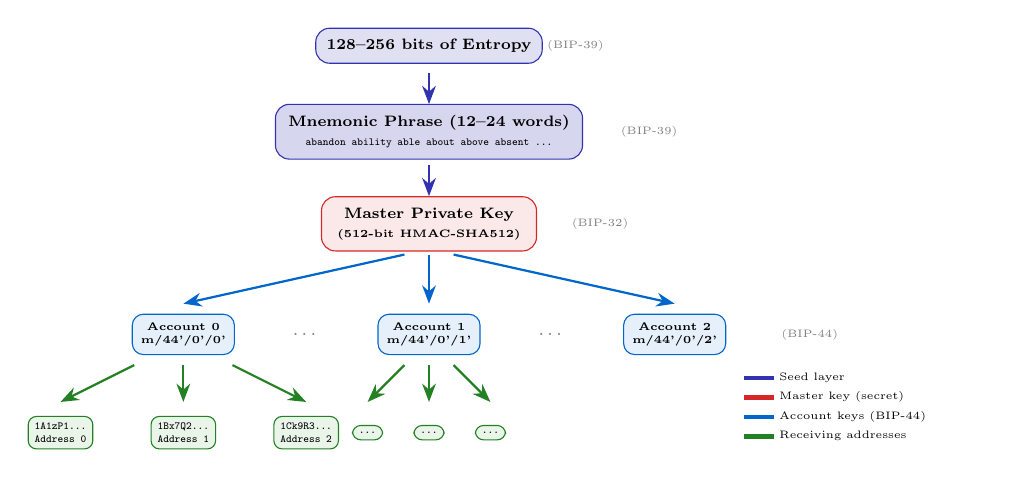
\begin{tikzpicture}[
  scale=0.78,
  every node/.style={transform shape},
  level/.style={font=\tiny},
  >=Stealth
]

% --- Level 0: Entropy / Seed ---
\node[draw=mlpurple, fill=mlpurple!15, rounded corners=5pt,
      font=\scriptsize\bfseries, inner sep=5pt, minimum width=3cm]
      (entropy) at (0,4.0) {128--256 bits of Entropy};
\node[font=\tiny, mlgray, right] at (1.8,4.0) {(BIP-39)};

% Arrow down
\draw[->, mlpurple, thick] (0,3.55) -- (0,3.05);

% --- Level 1: Mnemonic ---
\node[draw=mlpurple, fill=mllavender4, rounded corners=5pt,
      font=\scriptsize\bfseries, inner sep=5pt, minimum width=5cm, align=center]
      (mnemonic) at (0,2.6) {Mnemonic Phrase (12--24 words)\\[1pt]
      \tiny\ttfamily abandon ability able about above absent ...};
\node[font=\tiny, mlgray, right] at (3.0,2.6) {(BIP-39)};

% Arrow down
\draw[->, mlpurple, thick] (0,2.05) -- (0,1.55);

% --- Level 2: Master Key ---
\node[draw=mlred, fill=mlred!10, rounded corners=5pt,
      font=\scriptsize\bfseries, inner sep=5pt, minimum width=3.5cm, align=center]
      (master) at (0,1.1) {Master Private Key\\[1pt]\tiny (512-bit HMAC-SHA512)};
\node[font=\tiny, mlgray, right] at (2.2,1.1) {(BIP-32)};

% Branch to child keys
\draw[->, mlblue, thick] (-0.4,0.6) -- (-4.0,-0.2);
\draw[->, mlblue, thick] (0,0.6) -- (0,-0.2);
\draw[->, mlblue, thick] (0.4,0.6) -- (4.0,-0.2);

% --- Level 3: Child Keys (Accounts) ---
\node[draw=mlblue, fill=mlblue!10, rounded corners=4pt,
      font=\tiny\bfseries, inner sep=4pt, align=center]
      (child0) at (-4.0,-0.7) {Account 0\\m/44'/0'/0'};

\node[draw=mlblue, fill=mlblue!10, rounded corners=4pt,
      font=\tiny\bfseries, inner sep=4pt, align=center]
      (child1) at (0,-0.7) {Account 1\\m/44'/0'/1'};

\node[draw=mlblue, fill=mlblue!10, rounded corners=4pt,
      font=\tiny\bfseries, inner sep=4pt, align=center]
      (child2) at (4.0,-0.7) {Account 2\\m/44'/0'/2'};

\node[font=\tiny, mlgray] at (6.2,-0.7) {(BIP-44)};

% Dots between accounts
\node[font=\small, mlgray] at (-2.0,-0.7) {\ldots};
\node[font=\small, mlgray] at (2.0,-0.7) {\ldots};

% Branch to addresses from Account 0
\draw[->, mlgreen!80!black, thick] (-4.8,-1.2) -- (-6.0,-1.8);
\draw[->, mlgreen!80!black, thick] (-4.0,-1.2) -- (-4.0,-1.8);
\draw[->, mlgreen!80!black, thick] (-3.2,-1.2) -- (-2.0,-1.8);

% --- Level 4: Addresses ---
\node[draw=mlgreen!80!black, fill=mlgreen!10, rounded corners=3pt,
      font=\tiny\ttfamily, inner sep=3pt, align=center]
      at (-6.0,-2.3) {1A1zP1...\\Address 0};

\node[draw=mlgreen!80!black, fill=mlgreen!10, rounded corners=3pt,
      font=\tiny\ttfamily, inner sep=3pt, align=center]
      at (-4.0,-2.3) {1Bx7Q2...\\Address 1};

\node[draw=mlgreen!80!black, fill=mlgreen!10, rounded corners=3pt,
      font=\tiny\ttfamily, inner sep=3pt, align=center]
      at (-2.0,-2.3) {1Ck9R3...\\Address 2};

% Branch to addresses from Account 1
\draw[->, mlgreen!80!black, thick] (-0.4,-1.2) -- (-1.0,-1.8);
\draw[->, mlgreen!80!black, thick] (0,-1.2) -- (0,-1.8);
\draw[->, mlgreen!80!black, thick] (0.4,-1.2) -- (1.0,-1.8);

\node[draw=mlgreen!80!black, fill=mlgreen!10, rounded corners=3pt,
      font=\tiny\ttfamily, inner sep=3pt] at (-1.0,-2.3) {\ldots};
\node[draw=mlgreen!80!black, fill=mlgreen!10, rounded corners=3pt,
      font=\tiny\ttfamily, inner sep=3pt] at (0,-2.3) {\ldots};
\node[draw=mlgreen!80!black, fill=mlgreen!10, rounded corners=3pt,
      font=\tiny\ttfamily, inner sep=3pt] at (1.0,-2.3) {\ldots};

% Legend on the right
\node[font=\tiny, align=left, text width=3.8cm, anchor=north west] at (5.0,-1.2) {%
\textcolor{mlpurple}{\rule{0.5cm}{2pt}} Seed layer\\[3pt]
\textcolor{mlred}{\rule{0.5cm}{2pt}} Master key (secret)\\[3pt]
\textcolor{mlblue}{\rule{0.5cm}{2pt}} Account keys (BIP-44)\\[3pt]
\textcolor{mlgreen!80!black}{\rule{0.5cm}{2pt}} Receiving addresses};

\end{tikzpicture}
\end{center}
\bottomnote{Hierarchical Deterministic (HD) wallets derive unlimited addresses from a single seed -- back up once, recover everything.}
\end{frame}

% ==================== FRAME 8: REAL-WORLD ATTACKS ====================
\begin{frame}{Real-World Attacks on Cryptography}
\begin{center}
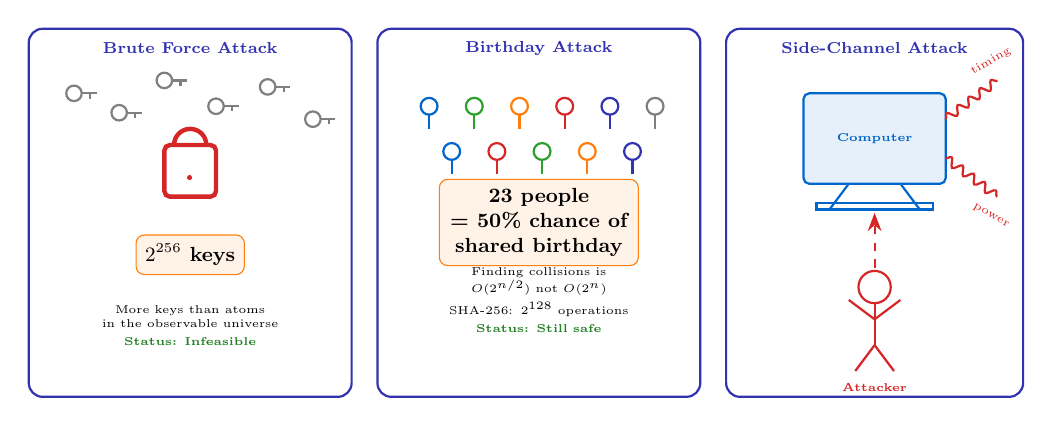
\begin{tikzpicture}[scale=0.82, every node/.style={transform shape}]

% ===== PANEL 1: Brute Force =====
\draw[mlpurple, thick, rounded corners=5pt] (-7.2,-2.5) rectangle (-2.2,3.2);
\node[font=\scriptsize\bfseries, mlpurple] at (-4.7,2.9) {Brute Force Attack};

% Keys raining down
\foreach \x/\y in {-6.5/2.2, -5.8/1.9, -5.1/2.4, -4.3/2.0, -3.5/2.3, -2.8/1.8} {
  \draw[mlgray, thick] (\x,\y) circle (0.12);
  \draw[mlgray, thick] (\x+0.12,\y) -- (\x+0.35,\y);
  \draw[mlgray, thick] (\x+0.25,\y) -- (\x+0.25,\y-0.08);
}

% Lock
\draw[mlred, ultra thick, rounded corners=2pt] (-5.1,0.6) rectangle (-4.3,1.4);
\draw[mlred, ultra thick] (-4.95,1.4) arc (180:0:0.25);
\node[font=\tiny, mlred] at (-4.7,0.9) {\textbullet};

% Number
\node[draw=mlorange, fill=mlorange!10, rounded corners=3pt,
      font=\small\bfseries, inner sep=4pt] at (-4.7,-0.3) {$2^{256}$ keys};

\node[font=\tiny, align=center, text width=3.5cm] at (-4.7,-1.4) {%
More keys than atoms\\in the observable universe\\[2pt]
\textcolor{mlgreen!80!black}{\bfseries Status: Infeasible}};

% ===== PANEL 2: Birthday Attack =====
\draw[mlpurple, thick, rounded corners=5pt] (-1.8,-2.5) rectangle (3.2,3.2);
\node[font=\scriptsize\bfseries, mlpurple] at (0.7,2.9) {Birthday Attack};

% People icons (simplified)
\foreach \x/\y/\c in {-1.0/2.0/mlblue, -0.3/2.0/mlgreen, 0.4/2.0/mlorange,
                       1.1/2.0/mlred, 1.8/2.0/mlpurple, 2.5/2.0/mlgray,
                       -0.65/1.3/mlblue, 0.05/1.3/mlred, 0.75/1.3/mlgreen,
                       1.45/1.3/mlorange, 2.15/1.3/mlpurple} {
  \draw[\c, thick] (\x,\y) circle (0.13);
  \draw[\c, thick] (\x,\y-0.13) -- (\x,\y-0.35);
}

% 23 people fact
\node[draw=mlorange, fill=mlorange!10, rounded corners=3pt,
      font=\small\bfseries, inner sep=4pt, text width=2.8cm, align=center]
      at (0.7,0.2) {23 people\\= 50\% chance of\\shared birthday};

\node[font=\tiny, align=center, text width=3.5cm] at (0.7,-1.0) {%
Finding collisions is\\$O(2^{n/2})$ not $O(2^n)$\\[2pt]
SHA-256: $2^{128}$ operations\\[2pt]
\textcolor{mlgreen!80!black}{\bfseries Status: Still safe}};

% ===== PANEL 3: Side-Channel =====
\draw[mlpurple, thick, rounded corners=5pt] (3.6,-2.5) rectangle (8.2,3.2);
\node[font=\scriptsize\bfseries, mlpurple] at (5.9,2.9) {Side-Channel Attack};

% Computer
\draw[mlblue, thick, fill=mlblue!10, rounded corners=2pt] (4.8,0.8) rectangle (7.0,2.2);
\node[font=\tiny\bfseries, mlblue] at (5.9,1.5) {Computer};
\draw[mlblue, thick] (5.5,0.8) -- (5.2,0.4);
\draw[mlblue, thick] (6.3,0.8) -- (6.6,0.4);
\draw[mlblue, thick] (5.0,0.4) rectangle (6.8,0.5);

% Spy with antenna
\draw[mlred, thick] (5.9,-0.8) circle (0.25);
\draw[mlred, thick] (5.9,-1.05) -- (5.9,-1.7);
\draw[mlred, thick] (5.9,-1.3) -- (5.5,-1.0);
\draw[mlred, thick] (5.9,-1.3) -- (6.3,-1.0);
\draw[mlred, thick] (5.9,-1.7) -- (5.6,-2.1);
\draw[mlred, thick] (5.9,-1.7) -- (6.2,-2.1);
\node[font=\tiny\bfseries, mlred] at (5.9,-2.35) {Attacker};

% Emanation waves
\draw[mlred, thick, decorate, decoration={snake, amplitude=1.5pt, segment length=5pt}]
     (7.0,1.8) -- (7.8,2.4);
\draw[mlred, thick, decorate, decoration={snake, amplitude=1.5pt, segment length=5pt}]
     (7.0,1.2) -- (7.8,0.6);
\node[font=\tiny, mlred, rotate=30] at (7.7,2.7) {timing};
\node[font=\tiny, mlred, rotate=-30] at (7.7,0.3) {power};

% Spy arrow
\draw[-{Stealth}, mlred, dashed, thick] (5.9,-0.5) -- (5.9,0.35);

\node[font=\tiny, align=center, text width=3.2cm] at (5.9,-1.0) {};

\end{tikzpicture}
\end{center}
\bottomnote{Defense in depth: use constant-time algorithms, hardware security modules, and key rotation to mitigate side-channel risks.}
\end{frame}

% ==================== FRAME 9: CRYPTO BY THE NUMBERS (pgfplots chart) ====================
\begin{frame}{Crypto by the Numbers: Key Size vs.\ Security}
\begin{columns}[T]
\begin{column}{0.58\textwidth}
\begin{center}
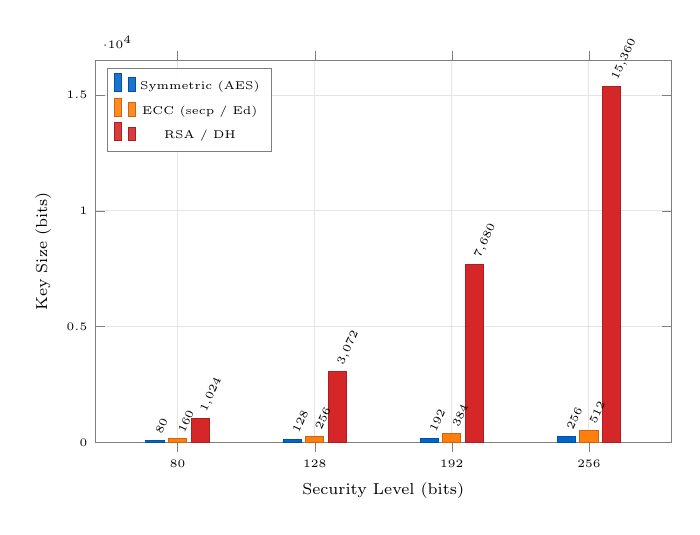
\begin{tikzpicture}[scale=0.82, every node/.style={transform shape}]
\begin{axis}[
    ybar,
    bar width=8pt,
    width=10.5cm,
    height=7.5cm,
    ylabel={Key Size (bits)},
    xlabel={Security Level (bits)},
    ymin=0,
    ymax=16500,
    symbolic x coords={80, 128, 192, 256},
    xtick=data,
    legend style={
      at={(0.02,0.98)},
      anchor=north west,
      font=\tiny,
      draw=mlgray,
      fill=white,
      fill opacity=0.9,
      text opacity=1,
    },
    ylabel style={font=\scriptsize},
    xlabel style={font=\scriptsize},
    tick label style={font=\tiny},
    nodes near coords,
    every node near coord/.append style={font=\tiny, rotate=65, anchor=west},
    enlarge x limits=0.2,
    grid=major,
    grid style={mlgray!20},
    axis line style={mlgray},
    major tick style={mlgray},
]

% Symmetric (AES)
\addplot[fill=mlblue, draw=mlblue!80!black] coordinates {
    (80, 80) (128, 128) (192, 192) (256, 256)
};

% ECC (ECDSA / secp)
\addplot[fill=mlorange, draw=mlorange!80!black] coordinates {
    (80, 160) (128, 256) (192, 384) (256, 512)
};

% RSA / DH
\addplot[fill=mlred, draw=mlred!80!black] coordinates {
    (80, 1024) (128, 3072) (192, 7680) (256, 15360)
};

\legend{Symmetric (AES), ECC (secp / Ed), RSA / DH}
\end{axis}
\end{tikzpicture}
\end{center}
\end{column}
\begin{column}{0.40\textwidth}
\vspace{3mm}
\begin{block}{\small Key Insight}
ECC achieves the \textbf{same security} as RSA with \textbf{much smaller keys}:
\begin{itemize}\setlength\itemsep{3pt}
\item[\textcolor{mlblue}{\textbullet}] AES-128: \textbf{128} bits
\item[\textcolor{mlorange}{\textbullet}] ECDSA-256: \textbf{256} bits
\item[\textcolor{mlred}{\textbullet}] RSA-3072: \textbf{3072} bits
\end{itemize}
All provide $\sim$\textbf{128-bit security}.
\end{block}

\vspace{2mm}
\begin{block}{\small Why Blockchain Uses ECC}
\begin{itemize}\setlength\itemsep{2pt}
\item Smaller keys $\to$ smaller transactions
\item Faster signing and verification
\item Lower bandwidth and storage
\item Bitcoin: \textbf{secp256k1}
\item Ethereum: also secp256k1
\end{itemize}
\end{block}

\vspace{2mm}
{\scriptsize\textcolor{mlred}{\bfseries Quantum threat:} Shor's algorithm could break ECC and RSA. Post-quantum research is ongoing.}
\end{column}
\end{columns}
\bottomnote{Source: NIST SP 800-57 key management recommendations. All three columns at 128-bit security are equivalent in strength.}
\end{frame}

% ==================== FRAME 10: TAKEAWAYS & CRYPTO PRINCIPLES ====================
\begin{frame}{Takeaways \& Crypto Principles}
\begin{columns}[T]
\begin{column}{0.55\textwidth}
\begin{block}{\normalsize Five Core Principles}
\begin{itemize}\setlength\itemsep{5pt}
\item \textcolor{mlgreen!80!black}{\bfseries$\checkmark$}
  \textbf{Hash functions} create tamper-evident fingerprints\\
  {\scriptsize SHA-256 secures every Bitcoin block}

\item \textcolor{mlgreen!80!black}{\bfseries$\checkmark$}
  \textbf{Asymmetric cryptography} enables trustless identity\\
  {\scriptsize No central authority needed to verify who you are}

\item \textcolor{mlgreen!80!black}{\bfseries$\checkmark$}
  \textbf{Digital signatures} prove ownership and intent\\
  {\scriptsize Every transaction is mathematically signed}

\item \textcolor{mlgreen!80!black}{\bfseries$\checkmark$}
  \textbf{Key management} is the weakest link in practice\\
  {\scriptsize ``Not your keys, not your coins''}

\item \textcolor{mlgreen!80!black}{\bfseries$\checkmark$}
  \textbf{Security is measured in bits}, not algorithms\\
  {\scriptsize 128-bit security is the current standard}
\end{itemize}
\end{block}
\end{column}
\begin{column}{0.43\textwidth}
\begin{block}{\normalsize Summary}
\begin{center}
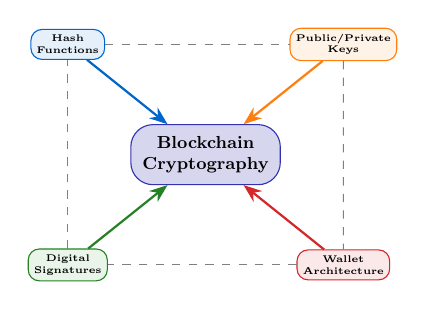
\begin{tikzpicture}[scale=0.7, every node/.style={transform shape}]

% Central node
\node[draw=mlpurple, fill=mllavender4, rounded corners=8pt,
      font=\small\bfseries, inner sep=6pt, minimum width=2.5cm,
      align=center] (center) at (0,0) {Blockchain\\Cryptography};

% Surrounding nodes
\node[draw=mlblue, fill=mlblue!10, rounded corners=4pt,
      font=\tiny\bfseries, inner sep=3pt, align=center] (hash) at (-2.5,2.0) {Hash\\Functions};
\node[draw=mlorange, fill=mlorange!10, rounded corners=4pt,
      font=\tiny\bfseries, inner sep=3pt, align=center] (keys) at (2.5,2.0) {Public/Private\\Keys};
\node[draw=mlgreen!80!black, fill=mlgreen!10, rounded corners=4pt,
      font=\tiny\bfseries, inner sep=3pt, align=center] (sig) at (-2.5,-2.0) {Digital\\Signatures};
\node[draw=mlred, fill=mlred!10, rounded corners=4pt,
      font=\tiny\bfseries, inner sep=3pt, align=center] (wallet) at (2.5,-2.0) {Wallet\\Architecture};

% Connections
\draw[-{Stealth}, mlblue, thick] (hash) -- (center);
\draw[-{Stealth}, mlorange, thick] (keys) -- (center);
\draw[-{Stealth}, mlgreen!80!black, thick] (sig) -- (center);
\draw[-{Stealth}, mlred, thick] (wallet) -- (center);

% Cross connections
\draw[mlgray, thin, dashed] (hash) -- (keys);
\draw[mlgray, thin, dashed] (keys) -- (wallet);
\draw[mlgray, thin, dashed] (wallet) -- (sig);
\draw[mlgray, thin, dashed] (sig) -- (hash);

\end{tikzpicture}
\end{center}
\end{block}

\vspace{2mm}
{\scriptsize\textcolor{mlpurple}{\bfseries Next lecture:} Consensus mechanisms -- how do thousands of nodes agree without a leader?}
\end{column}
\end{columns}
\bottomnote{Cryptography is the mathematical foundation that makes decentralized trust possible.}
\end{frame}

\end{document}
